\chapter{战术导弹制导控制系统分析与设计}
\section{制导回路设计}
\subsubsection{制导回路开环增益}
由于校正网络使用的超前-滞后校正,不会含有积分环节,因而大回路的开环增益可以由输入输出决定:
$$K_{ol\ min}=\frac{f_{y\ max}}{\Delta y_{max}}$$
脱靶量$\Delta y_{max}$由技术战术指标确定,最大需用法向过载$f_{y\ max}$由导引弹道分析给出。
对于指令制导的导弹,前馈的部分期望法向过载直接由基站计算得出,
而且这一部分的期望加速度在总期望加速度中占比很大。制导回路的主要作用是消除较小的偏差。这里的主要工作
应该放在指导指令的计算以及执行的精确性上。
\subsubsection{制导回路开环截止频率}
自动驾驶仪回路的弹体固有频率(带宽)不小于开环截止频率的4-5倍。保证稳定性的前提,{\kaishu 导弹必须有
足够的能力执行外环的指令}
\subsubsection{校正网络作用于制导回路}
本部分是制导回路的校正网络设计:

三点法当中,若不考虑自动驾驶仪回路,那么制导回路至少是一个2型系统,此时的系统至多是临界稳定的,(-180°)
三点法主要用到的校正网络类型:
PID控制器和超前滞后校正网络:(网络特性略)

{\heiti 校正网络设计:}

假设自动驾驶仪回路的增益为$K_W$,制导回路开环增益已经选定:

超前-滞后校正网络设计:
主要任务是设计分度系数a以及时间常数T,a决定了最大超前角$\varphi_m$,T决定了校正网络的位置。最大超前角由需要确定。
PID控制器设计:
KI和KD由设计给出,KP由仿真给出。制导回路开环截止频率:$\omega_c = K_WK_D$,增益:$K_{OL}=K_WK_I$,PID控制器
在低频与高频增益变大,因为积分与微分作用的存在,因而需要让$\sqrt{\frac{K_I}{K_D}}=\omega_{pid} < \frac{1}{\xi}\omega_c$,发挥出
超前校正以及积分消除静差作用。
\section{过载自动驾驶仪分析设计}
前面提到了自动驾驶仪回路的弹体固有频率(带宽)不小于开环截止频率的4-5倍,从频率分析角度,实际上将自动驾驶仪的
截止频率“往后放”,减小整体带来的相位滞后。

\subsection{矛盾}
\begin{enumerate}
    \item 高的命中精度,要求制导大回路开环增益大,\textcolor{green}{??制导回路开环截止频率较大(往上抬了,对对对)},导致要求弹体固有频率也得提高,但是提高受限。
    \item 弹体的固有频率需要比较高(外环要求),不能把静稳定度放的太大,导致弹体增益太低,舵机系统压力太大
    \item 静稳定度太大,导致阻尼太小,会直接产生一堆问题:例如射程降低,超调震荡之类。
\end{enumerate}
\subsection{自驾仪特性分析}
\begin{figure}[H]
    \centering
    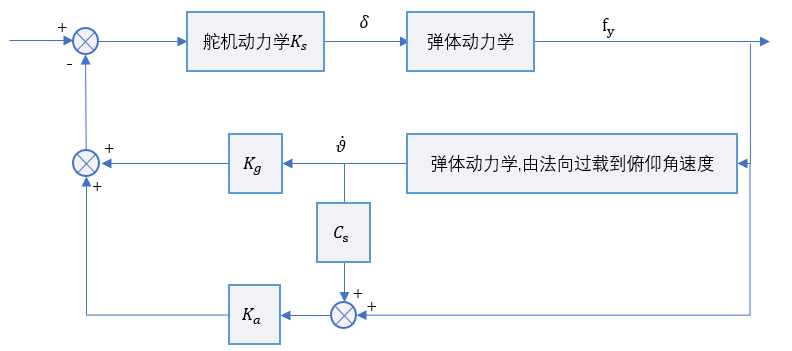
\includegraphics[scale = 0.7]{pictures/chapter10/1}
    \caption{自驾仪结构}
    \label{autopliot}
\end{figure}

{\heiti 自驾仪回路指标与参数关系:}

\begin{enumerate}
    \item 自驾仪稳态增益:$K_{au} = \frac{1}{K_a+\frac{K_g}{V}}$,开环增益足够大时,
    自驾仪的稳态增益基本与弹体动力学无关。
    \item $K_g$用来调节阻尼
    \item $K_a$和$K_s$来确定自驾仪的开环增益:
    
    {\kaishu $\omega_{au} = \sqrt{-K_aK_sVa_{25}a_{24}}$,且二阶系统的固有频率与无阻尼自然频率成正比
    ,因而,$K_a\times K_s$可确定自驾仪的固有频率}
    \item 自驾仪反馈的恰好是法向过载以及俯仰角速度,这就是忽略舵机动力学条件下的全状态反馈,可以实现零极点任意配置
    \item 自驾仪不能忽略舵机动力学的时候变成了输出反馈
    \item 自驾仪反馈的是俯仰角速度增大阻尼,其实和反馈法向过载变化率作用基本一致
    \item 当自驾仪开环增益过大时,开环截止频率将基本和舵机固有频率一致,这使得反馈回路的校正能力捉襟见肘
\end{enumerate}
\subsection{自驾仪设计步骤}
\begin{enumerate}
    \item 制导回路开环截止频率设计自驾仪带宽(其实和已知自驾仪开环截止频率选舵机带宽的思路是一致的)
    
    {\kaishu 遵循4-5倍的原则}
    \item 自驾仪带宽确定舵机带宽
    
    {\kaishu 自驾仪的开环截止频率与带宽十分接近,要使舵机带宽大于3-4倍。
    阻尼按照一般的控制系统设计原则选取。}
    \item 初选$K_a$,根据带宽约束选择$K_s$,
    
    {\kaishu 这里的$K_g$对于自然频率影响很小,给为0;绘制$K_s$的开环根轨迹,选取合适的值}
    \item 确定阻尼回路增益$K_g$
    
    {\kaishu 这里的$K_g$增大时,低频模态稳定性加强,高频降低}

    \item 校核开环增益
\end{enumerate}




